\documentclass[a4paper,11pt]{bxjsarticle}
\usepackage{xltxtra}
\usepackage{zxjatype}
\usepackage{here}
\setjamainfont[BoldFont=ipaexm.ttf]{ipaexm.ttf}
\setjasansfont[BoldFont=ipaexg.ttf]{ipaexg.ttf}
\usepackage{enumitem}
\usepackage{amsmath}
\usepackage{amssymb}
\usepackage{booktabs}
\usepackage{listings}
\usepackage{bm}
\usepackage{cite} 
\newtheorem{mf}{公式}

\lstset{
basicstyle={\scriptsize}
}
\setlist[enumerate]{listparindent=2pt}


\begin{document}
\begin{titlepage}
  \begin{center}
    \vspace*{150truept}
    {\Huge 微分方程式}\\ % タイトル
    \vspace{120truept}
    {\huge 18T1694W}\\ % 学籍番号
    \vspace{50truept}
    {\huge 島袋 隆也}\\ % 著者
    \vspace{50truept}
    {\huge \today}\\ % 提出日
  \end{center}
\end{titlepage}


%=====================================================================

%=====================================================================
\section{公式}
計算に使う公式を以下に示す.
\begin{mf}
  $\frac{1}{D+\alpha}r(x) = e^{-\alpha x}\int r(x)e{\alpha x}$
  \label{mf:1}
\end{mf}
\begin{mf}
  $y_p=\frac{1}{P(D)}e^{\alpha x} = \frac{1}{P(\alpha)}e^{\alpha x}, (P(\alpha)\neq 0)$
  \label{mf:2}
\end{mf}

          

%=====================================================================
\section{大問1}
問題文を以下に示す.
\subsection{問1|$y''-2y'-3y=e^x$}
問題文の式は以下の特徴をもつ.

\begin{itemize}
  \item $y''$が最も高い階数→2階
  \item $y$の微分係数に$x$がかかっていない → 定数係数
  \item $y''$にかかる係数が1 → 正規系
  \item $y$と$y$の微分がすべて1乗 → 線形
  \item $e^x$が存在 → 非斉次
\end{itemize}

上記により線形非斉次微分方程式であることがわかる.\\
線形非斉次微分方程式において,演算子法を用いた特解の導出は以下の手順で行う.

\begin{enumerate}
  \item 演算子法を用いて表す.
  \item yについて解く.
  \item 変形した逆演算子を用いる.
\end{enumerate}

微分演算子を用い,$y_p$の式に直すと以下のようになる.

\begin{equation}
  y_p = \frac{1}{(D^2-2D-3)}e^x
\end{equation}

ここで,$(P(1)=-4\neq 0)$が成り立つため,公式(\ref{mf:2})を用いることができる.
よって特解$y_p$は以下のように求まる.

\begin{equation}
  y_p = -\frac{1}{4}e^{x}
\end{equation}

\subsection{問2|$y''-2y'-3y=e^{3x}$}
問2も問1と同様に線形非斉次微分方程式である.
よって,微分演算子を用い,因数分解し,特解$y_p$の式に直すと以下のようになる.

\begin{equation}
  y_p = \frac{1}{(D-3)(D+1)}e^{3x}
\end{equation}

ここで,$(P(3)= 0)$より公式(\ref{mf:2})が使えない.
そこで,基本公式である公式(\ref{mf:1})を用いると

\begin{equation}
  \frac{1}{D-3}\cdot\frac{1}{4}e^{3x}
\end{equation}

となり,特解$y_p$は以下のように求まる.

\begin{equation}
  y_p=\frac{1}{4}xe^{3x}
\end{equation}

\subsection{問3|$y''-2y'-3y=e^x+e^{3x}+\sin x$}
非斉次項の$\sin x$はオイラーの公式を応用し$e_{ix}$と置き換えられる.
問2と同様に計算すると,特解$y_p$を求める式は以下のようになる.

\begin{equation}
  y_p = \frac{1}{(D - 3)(D + 1)}(e^x + e^{3x} + e^{ix})
\end{equation}

公式(\ref{mf:1})を用いると,

\begin{equation}
  y_p = \frac{1}{D - 3}(\frac{1}{2}e^x + \frac{1}{4}e^{3x} + \frac{1}{1+i}e^{ix})
\end{equation}

同様に$\frac{1}{D-3}$の項も計算し,$e^{ix}$の係数を有理化すると,

\begin{equation}
  y_p = -\frac{1}{4}e^x + \frac{1}{4}xe^{3x} - \frac{2 - i}{10}(\cos x + i\sin x)
\end{equation}

ここで,$\sin x$を$e^{ix}$と置いたことから虚部を解にすると特解$y_p$は以下のように求まる.

\begin{equation}
  y_p = -\frac{1}{4}e^x + \frac{1}{4}xe^{3x} - \frac{1}{5}\sin x + \frac{1}{10}\cos x
\end{equation}

\section{大問2}
式(\ref{equ:2-1})について,以下について答えよ.

\begin{equation}
  \frac{d^2x}{dt^2}+\alpha \frac{dx}{dt}+x=F(t) (\alpha \geq 0)
  \label{equ:2-1}
\end{equation}

\subsection{問1|特性方程式の解が虚数解となる定数$\alpha$の範囲を求めよ}
式(\ref{equ:2-1})の特性方程式は以下のようになる.

\begin{equation}
  \lambda^2 + \alpha \lambda + x = 0
\end{equation}

二次方程式の解の公式を用いると,

\begin{equation}
 \lambda = \frac{-\alpha \pm \sqrt{\alpha^2 - 4}}{2}
 \label{equ:2-2}
\end{equation}

よって,虚数解となる$\alpha$の範囲は$()\alpha \geq 0)$であることを考慮し,
\begin{equation}
  0 \leq \alpha < 2
\end{equation}

\subsection{問2|$\alpha=0$のときの斉次解を求めよ。}
式(\ref{equ:2-2})に$\alpha=0$を代入して特性方程式の解を求めると,斉次解は
\begin{equation}
  x= C_1e^{it}+C_2e^{-it}, 
\end{equation}
で与えられる.($C_1$, $C_2$は任意定数)

ここで,オイラーの公式を用い,$A=i(C_1-C_2),B=C_1+C_2$とすると
\begin{equation}
  y= A\sin t + B\cos t, 
\end{equation}

で与えられる.(A,Bは任意定数)

\subsection{問3|$\alpha=0$, $F(t)=2\cos t$ のときの一般解を求めよ。}
斉次解は問2で求めてあるため,特解を求める.
微分演算子を用いて大問1の問2と同様に計算すると
\begin{equation}
  x_p=\frac{1}{(D-i)(D+i)}2e^{it}=t\sin t
\end{equation}

よって,一般解は

\begin{equation}
  x = A\sin t + B\cos t + t\sin t
\end{equation}

ここで考察を述べていく.この問題は,質量$m=1$,摩擦係数$\alpha,(\alpha \geq 0)$,ばね係数$k=1$の重りがついた
バネに,外力$2\cos x$が加わっているものと考えることができる.\\
外力を$2\cos x$,内力を$x'' + \alpha x' + x$とし,特性方程式から推測できる3つの条件でそれぞれ場合分けして考える.
\newpage
\underline{$\alpha=2$}\\
これは臨界値であり,外力と内力が釣り合っている状態である.
そのため,時間が経つと振動はするが振幅は変わらない.グラフに描くと図\ref{fig:2}のようになる.

\begin{figure}[!htbp]
  \centering  % 図を真ん中に配置
  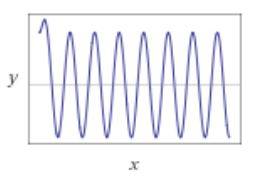
\includegraphics[clip,width = 4.0cm]{2.jpg}
  \caption{$\alpha=2$のときのグラフ}
  \label{fig:2}
  \end{figure}

\underline{$\alpha <2$}\\
これは,外力が内力を上回っている様態であり,時間が経つと振動しながら振幅が大きくなる.グラフに描くと図\ref{fig:0}のようになる.
\begin{figure}[htbp]
  \centering  % 図を真ん中に配置
  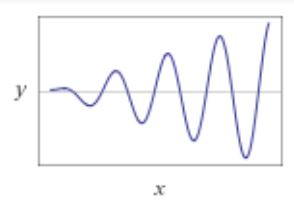
\includegraphics[clip,width = 4.0cm]{0.jpg}
  \caption{$\alpha=0$のときのグラフ}
  \label{fig:0}
  \end{figure}

\underline{$\alpha >2$}\\
これは,内力が外力を上回っている状態であり,時間がたつと振動しながら減衰していきやがて,$2cos x$に収束する
動きを見せる.グラフに描くと図\ref{fig:10}のようになる.
\begin{figure}[htbp]
  \centering  % 図を真ん中に配置
  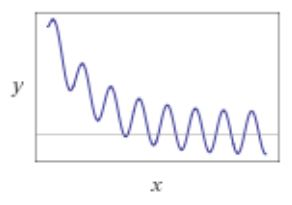
\includegraphics[clip,width = 4.0cm]{10.jpg}
  \caption{$\alpha=10$のときのグラフ}
  \label{fig:10}
  \end{figure}
%=====================================================================


\end{document}
